\section{Мутагенез. Спонтанный мутагенез. Скорость мутагенеза.
Индуцированный мутагенез. Репарация димеров тимина с помощью фотолиазы и эксцизионной репарации.
Понятие сайт-специфического мутагенеза.}
	
\subsection{Мутагенез. Естественный мутагенез - Мутационная теория Де Фриза и Коржинского}

Мутагенез — процесс изменения в нуклеотидной последовательности ДНК, приводящий к мутациям. \\

Мутационная теория составляет одну из основ генетики. В ее основу были заложены идеи Де Фриза и Коржинского.

Основные положения мутационной теории Коржинского — Де Фриза можно свести к следующим пунктам (кратко):

\begin{enumerate}
	\item Мутации внезапны, как дискретные изменения признаков
	Новые формы устойчивы
	\item В отличие от наследственных изменений, мутации не образуют непрерывных рядов, не группируются вокруг какого-либо среднего типа. Они представляют собой качественные скачки изменений
	\item Мутации проявляются по-разному и могут быть как полезными, так и вредными
	\item Вероятность обнаружения мутаций зависит от числа исследуемых особей
	\item Сходные мутации могут возникать неоднократно
\end{enumerate}

\subsubsection{Механизмы мутагенеза}

Последовательность событий, приводящая к мутации выглядит следующим образом: происходит повреждение ДНК (если повреждение ДНК не было корректно репарировано, оно приведет к мутации); в случае, если повреждение произошло в незначащем фрагменте ДНК или если повреждение произошло в значащем фрагменте и, вследствие вырожденности генетического кода, не произошло нарушения, то мутации образуются, но их биологические последствия будут незначительными или могут не проявиться.

\subsection{Скорость мутагенеза}

Скорость мутагенеза - темп нуклеотидных замен. 

Как посчитать?\\

Один из самых простых способов - изучение родословных с целью подсчета вновь возникающих мутаций с четким фенотипическим эффектом и высокой пенетрантностью (то есть таких мутаций, которые меняют фенотип строго определенным образом и наверняка). Как правило, для этого используют мутации, вызывающие врожденные патологии, так как они  вызываются единичными мутациями.

\begin{figure}[H]
	\centering
	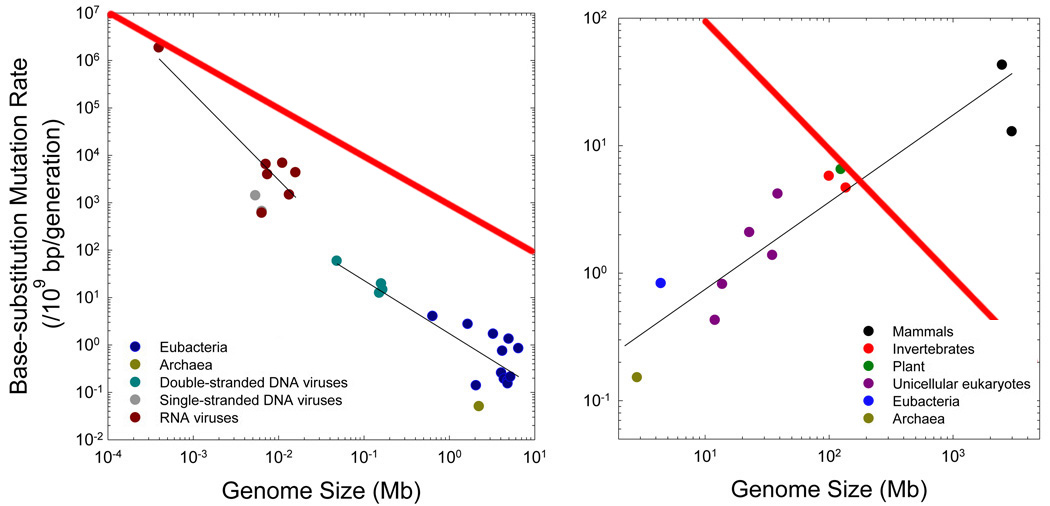
\includegraphics[width=0.7\linewidth]{7_mutation_pace}
	\caption{Скорость мутация, слева для вирусов и прокариот, справа для эукариот. По вертикали - темп нуклеотидных замен на миллиард пар оснований (bp - base-pair), по горизонтали - размер генома в миллионах оснований (Mb - Mega base). Вывод: для вирусов и прокариот чем сложнее организм, тем меньше скорость его мутагенеза, для эукариот - чем сложнее оргинзм, тем выше скорость его мутагенеза.}
	\label{7_mutation_pace}
\end{figure}
	
\subsection{Индуцированный мутагенез}

Искусственный мутагенез широко используют для изучения белков и улучшения их свойств. \\

\textbf{Ненаправленный мутагенез}

Методом ненаправленного мутагенеза в последовательность ДНК вносятся изменения с определённой вероятностью под воздействием мутагенных факторов — мутагенных веществ, ультрафиолета, радиации. \\

\textbf{Направленный мутагенез \ ПЦР - мутагенез}

Изменения в ДНК вносятся в заранее известный сайт. Для этого синтезируют короткие одноцепочечные молекулы ДНК (праймеры), комплементарные целевой ДНК за исключением места мутации. \\

\textbf{Вставной мутагенез}

Cоздание мутаций ДНК путем добавления одной или более пар оснований. \\

\subsection{Понятие сайт-специфического мутагенеза}

Сайт-направленный мутагенез является методом молекулярной биологии, который используется, чтобы создать конкретные и преднамеренные изменения в последовательности ДНК, гена и продуктов генов.

\begin{figure}[H]
	\centering
	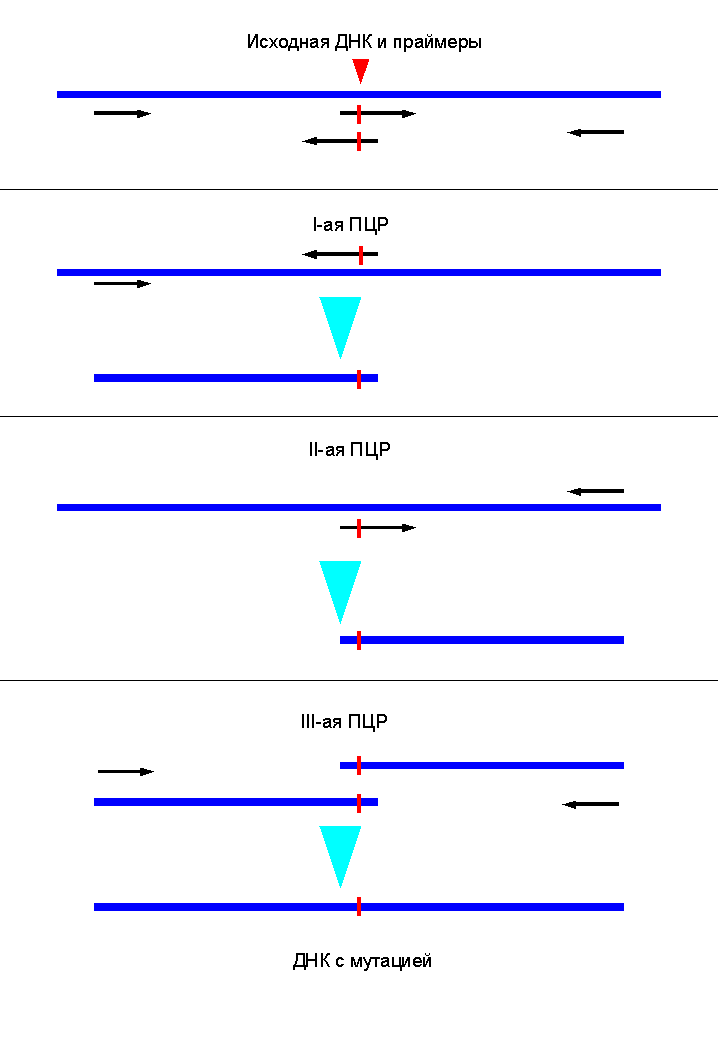
\includegraphics[width=0.7\linewidth]{7_site_mutagenesis}
	\caption{Сайт-направленный мутагенез. Синтезируют пару праймеров, несущих мутацию, и пару праймеров, комплементарных концам нужного фрагмента ДНК. В ходе первых двух реакций образуются фрагменты ДНК с мутацией, которые объединяют в третьей реакции. Полученный фрагмент вставляют в нужную генно-инженерную конструкцию.}
	\label{7_site_mutagenesis}
\end{figure}

\subsection{Репарация димеров тимина с помощью фотолиазы и эксцизионной репарации}

Пиримидиновый димер — дефект ДНК, возникающий в результате образования ковалентной связи между двумя соседними пиримидиновыми основаниями (тимином или цитозином) под действием ультрафиолетовых лучей. Ультрафиолетовые лучи вызывают разрыв двойной связи и образование в этом месте ковалентной связи между двумя нуклеотидами. Образование димера приводит к нарушению транскрипции ДНК на данном участке и возникновению мутаций.

\begin{figure}[H]
	\centering
	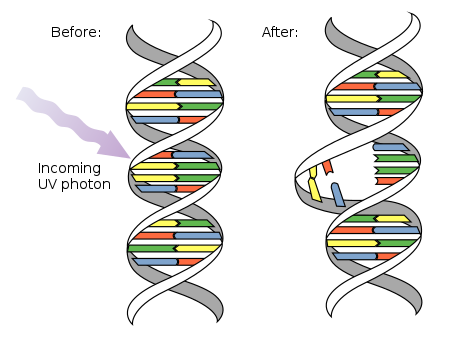
\includegraphics[width=0.7\linewidth]{7_dna_lesion}
	\caption{Дефект ДНК - димер тимина}
	\label{7_dna_lesion}
\end{figure}
	
\begin{figure}[H]
	\centering
	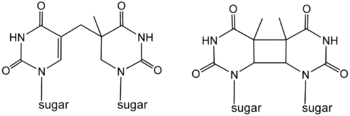
\includegraphics[width=0.7\linewidth]{7_timin_dimer}
	\caption{То, что образуется в результате дефекта. Слева: 6,4-фотопродукт. Справа: циклобутановый димер}
	\label{7_timin_dimer}
\end{figure}
	
\subsubsection{Репарация ДНК}

\textbf{ДНК-фотолиаза}

Один из способов удаления пиримидиновых димеров состоит в ферментативном превращении их в мономеры при освещении видимым светом в диапазоне длин волн 300—600 нм. ДНК-фотолиаза образует стабильный комплекс с пиримидиновым димером и, используя энергию поглощённого им света, разрушает димер без разрыва цепей ДНК. \\

\textbf{Эксцизионная репарация нуклеотидов}

Подразумевает удаление повреждённых азотистых оснований из ДНК и последующее восстановление нормальной структуры молекулы по комплементарной цепи. Ферментативная система удаляет короткую однонитевую последовательность двунитевой ДНК, содержащей поврежденные основания, и замещает их путём синтеза последовательности, комплементарной оставшейся нити. \\
